
%----------------------------------------------------------------------------------------
%	PACKAGES AND THEMES
%----------------------------------------------------------------------------------------

\documentclass{beamer}

\mode<presentation> {

% The Beamer class comes with a number of default slide themes
% which change the colors and layouts of slides. Below this is a list
% of all the themes, uncomment each in turn to see what they look like.

%\usetheme{default}
%\usetheme{AnnArbor}
%\usetheme{Antibes}
%\usetheme{Bergen}
%\usetheme{Berkeley}
%\usetheme{Berlin}
%\usetheme{Boadilla}
%\usetheme{CambridgeUS}
%\usetheme{Copenhagen}
%\usetheme{Darmstadt}
%\usetheme{Dresden}
%\usetheme{Frankfurt}
%\usetheme{Goettingen}
%\usetheme{Hannover}
%\usetheme{Ilmenau}
%\usetheme{JuanLesPins}
%\usetheme{Luebeck}
\usetheme{Madrid}
%\usetheme{Malmoe}
%\usetheme{Marburg}
%\usetheme{Montpellier}
%\usetheme{PaloAlto}
%\usetheme{Pittsburgh}
%\usetheme{Rochester}
%\usetheme{Singapore}
%\usetheme{Szeged}
%\usetheme{Warsaw}

% As well as themes, the Beamer class has a number of color themes
% for any slide theme. Uncomment each of these in turn to see how it
% changes the colors of your current slide theme.

%\usecolortheme{albatross}
%\usecolortheme{beaver}
%\usecolortheme{beetle}
%\usecolortheme{crane}
%\usecolortheme{dolphin}
%\usecolortheme{dove}
%\usecolortheme{fly}
%\usecolortheme{lily}
%\usecolortheme{orchid}
%\usecolortheme{rose}
%\usecolortheme{seagull}
%\usecolortheme{seahorse}
%\usecolortheme{whale}
%\usecolortheme{wolverine}

%\setbeamertemplate{footline} % To remove the footer line in all slides uncomment this line
%\setbeamertemplate{footline}[page number] % To replace the footer line in all slides with a simple slide count uncomment this line

\setbeamertemplate{navigation symbols}{} % To remove the navigation symbols from the bottom of all slides uncomment this line

\definecolor{water}{HTML}{3fb0ac}
\colorlet{beamer@blendedblue}{water}

\usebackgroundtemplate%
{
		
		 %  
\includegraphics[scale=0.5]{res/logo.png} 
		      
}

\setbeamertemplate{footline}
{
\vspace{1.5cm}
  \leavevmode%
  \hbox{%
    \begin{beamercolorbox}[wd=.9\paperwidth,ht=2.25ex,dp=1ex,center]{title in head/foot}%
      \usebeamerfont{title in head/foot}\pgfsetfillopacity{1}\insertshorttitle
    \end{beamercolorbox}%
    \begin{beamercolorbox}[wd=.1\paperwidth,ht=2.25ex,dp=1ex,right]{date in head/foot}%
      \insertframenumber{} / \inserttotalframenumber\hspace*{2ex}
    \end{beamercolorbox}}%
  \vskip0pt%
}



}

\usepackage{graphicx} % Allows including images
\usepackage{booktabs} % Allows the use of \toprule, \midrule and \bottomrule in tables
\usepackage[german]{babel}
\usepackage[utf8x]{inputenc}
\usepackage{textpos}
%----------------------------------------------------------------------------------------
%	TITLE PAGE
%----------------------------------------------------------------------------------------

\title[Autorisierungsmanagement für eine virtuelle
Forschungsumgebung für Geodaten: Qualitätssicherung]{Autorisierungsmanagement für eine virtuelle
Forschungsumgebung für Geodaten \\ \textbf{QUALITÄTSSICHERUNG}} % The short title appears at the bottom of every slide, the full title is only on the title page

\author[]{
Bachvarov, Aleksandar\\
Dimitrov, Atanas\\
Mortazavi Moshkenan, Houraalsadat\\
Sakly, Khalil\\
Slobodyanik, Anastasia\\
Voneva, Sonya
} % Your name

\institute[] % Your institution as it will appear on the bottom of every slide, may be shorthand to save space
{
Karlsruher Institut für Technologie % Your institution for the title page

}
\date{07. März 2018} % Date, can be changed to a custom date

\begin{document}

\begin{frame}[plain]
\titlepage % Print the title page as the first slide
\end{frame}


%----------------------------------------------------------------------------------------
%	PRESENTATION SLIDES
%----------------------------------------------------------------------------------------
\addtobeamertemplate{frametitle}{}{%
\begin{textblock*}{70mm}(.90\textwidth,-1cm)

\includegraphics[height=1cm,width=1cm]{res/logo}
\end{textblock*}}


\begin{frame}
\frametitle{Einleitung}
\framesubtitle{Testphasen}

\begin{center}
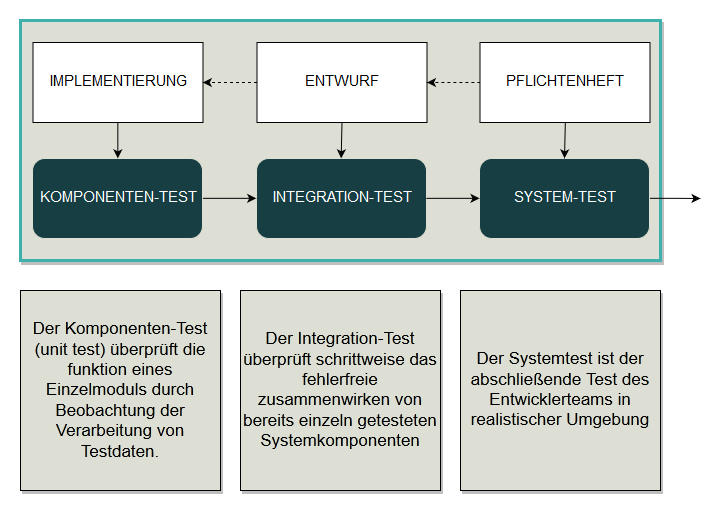
\includegraphics[height=\textheight]{res/testphasen.png}
\end{center}

\end{frame}
%------------------------------------------------
\begin{frame}

\frametitle{Komponenten-Test}
\framesubtitle{Unittests}
\begin{itemize}
\item<1-3> Eine Test-Klasse für jeden View
\item<2-3> Fallunterscheidung durch Methoden
\item<3> 21 Klassen, 91 Methoden
\end{itemize}


\end{frame}
%------------------------------------------------
\begin{frame}

\frametitle{Komponenten-Test}
\framesubtitle{Beispiel}
\begin{figure}
   \includegraphics<1>[width=\textwidth]{res/unittest.png}
   \includegraphics<2>[width=\textwidth]{res/unittest1.png}
   \includegraphics<3>[width=\textwidth]{res/unittest2.png}
   \includegraphics<4>[width=\textwidth]{res/unittest3.png}
\end{figure}

\end{frame}
%------------------------------------------------
\begin{frame}
\frametitle{Integration-Test}
\framesubtitle{Automatisierte Tests}

\begin{itemize}
\item<1-7> Django: Model-View-Template
\item<2-7> Konsistenz der Datenbank vor und nach den Benutzeraktionen
\item<3-7> 3 Test-Klassen entsprechend der Daten:
	\begin{itemize}
		\item<4-7> TestUserData
		\item<5-7> TestResourcesData
		\item<6-7> TestRequestsData
	\end{itemize}
\item<7>  14 Methoden überprüfen mögliche Szenarien, die die Datenbank beeinflussen können
\end{itemize}

\end{frame}
%------------------------------------------------
\begin{frame}
\frametitle{Integration-Test}
\framesubtitle{Beispiel}
\begin{figure}
   \includegraphics<1>[width=\textwidth]{res/integrationtest.png}
   \includegraphics<2>[width=\textwidth]{res/integrationtest1.png}
   \includegraphics<3>[width=\textwidth]{res/integrationtest2.png}
\end{figure}

\end{frame}
%------------------------------------------------

\begin{frame}
\frametitle{System-Test}
\framesubtitle{Manuelle Tests}

\begin{itemize}
\item<1-4> Pflichtenheft: Testfälle entsprechen funktioneller Anforderungen
\item<2-4> Szenarien: 
	\begin{itemize}
		\item<2-4> mehrere Benutzer
		\item<2-4> Real-time
		\item<2-4> Fehlerbenachrichtigungen
		\item<2-4> Fehlertoleranz \& Konsistenz
	\end{itemize}
\item<3-4>  Getestete Umgebung
		\begin{itemize}
		\item<3-4> Ubuntu
			\begin{itemize}
				\item<4> Firefox
			\end{itemize}
		\item<3-4> Windows
			\begin{itemize}
				\item<4> Firefox, Chrome, Opera, Edge
			\end{itemize}
		\item<3-4> Mac OS
			\begin{itemize}
				\item<4> Safari
			\end{itemize}
	\end{itemize}
\end{itemize}


\end{frame}
%------------------------------------------------

\begin{frame}
\frametitle{Fehler}
\begin{itemize}
		\item<1-3> Bugtracker im Trello
		\includegraphics<1>[width=\linewidth,height=\textheight,keepaspectratio]{res/bugtracker.png}
		\item<2-3> 16 Probleme (einige enthalten Gruppen von ähnlichen Fällen)
		\item<3> Fehlerbenachrichtigungen, Weiterleitungen, Textfelder
	\end{itemize}
\end{frame}

%------------------------------------------------

\begin{frame}
\frametitle{Codeüberdeckung}
\framesubtitle{Vor der Testphase}
\begin{center}
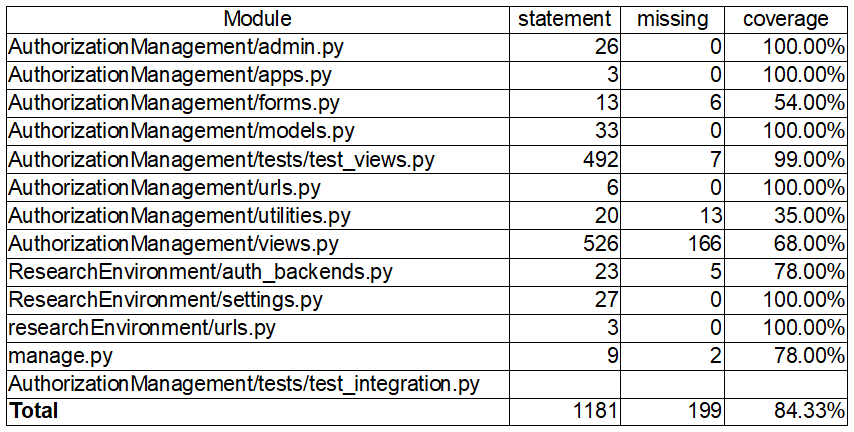
\includegraphics[scale=0.6]{res/coverage_before.png}
\end{center}
\end{frame}

%------------------------------------------------

\begin{frame}
\frametitle{Codeüberdeckung}
\framesubtitle{Nach der Testphase}
\begin{center}
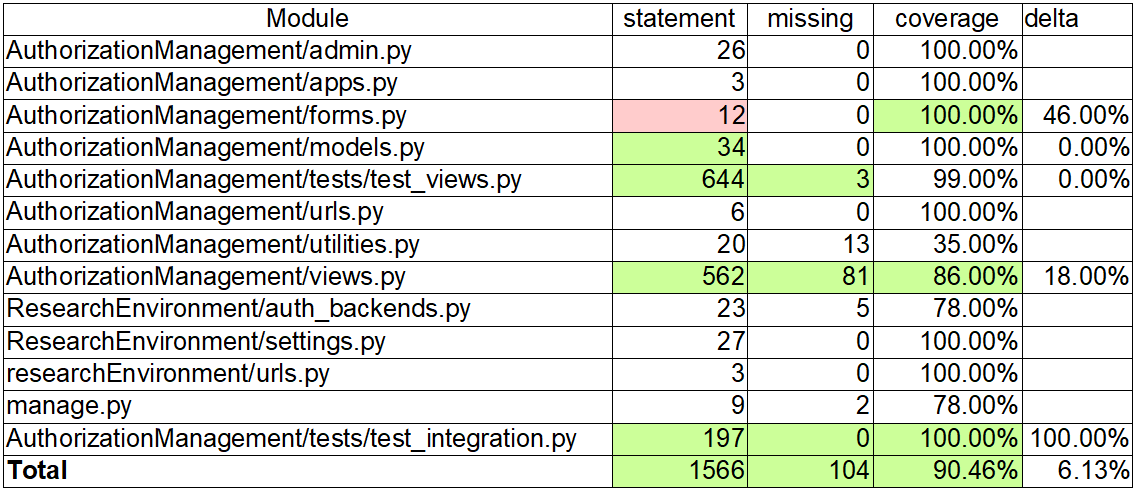
\includegraphics[scale=0.5]{res/coverage_after.png}
\end{center}
\end{frame}

%------------------------------------------------
\begin{frame}
\frametitle{Fazit}
	\begin{itemize}
		\item<1-4> 105 automatischen Tests
		\item<2-4> 90\% Codeüberdeckung
		\item<3-4> 25 manuellen Tests
		\item<4> Interne Abnahme\\
	
	\begin{center}
	Das Produkt ist somit fertig und \\bereit für Einsatz und Wartung.
	\end{center}
	
	\end{itemize}
\end{frame}

%------------------------------------------------
\begin{frame}
\frametitle{To be continued...}
	

 \begin{center}
	Unser Team wünscht Ihnen viel Spaß mit der AuthorizationManagement-App!
	\end{center}
	
\end{frame}

%----------------------------------------------------------------------------------------

\end{document}